\documentclass[  usegeometry% <- add this option
]{scrartcl}
\date{}
% \usepackage[margin=3.5cm
% %   ,showframe% <- only to show the page layout
% ]{geometry}
\reversemarginpar % Move the margin to the left of the page 
\usepackage{graphicx}
\usepackage{comment}
\pagenumbering{gobble}
\newcommand{\MarginText}[1]{\marginpar{\raggedleft\itshape\small#1}} % New command defining the margin text style

\usepackage[nochapters]{classicthesis} % Use the classicthesis style for the style of the document
\usepackage[LabelsAligned]{currvita} % Use the currvita style for the layout of the document

\renewcommand{\cvheadingfont}{\LARGE\color{Maroon}} % Font color of your name at the top

\usepackage{hyperref} % Required for adding links	and customizing them
\hypersetup{colorlinks, breaklinks, urlcolor=Maroon, linkcolor=Maroon} % Set link colors

\newlength{\datebox}\settowidth{\datebox}{Spring 2011} % Set the width of the date box in each block

\newcommand{\NewEntry}[3]{\noindent\hangindent=2em\hangafter=0 \parbox{\datebox}{\small \textit{#1}}\hspace{1.5em} #2 #3 % Define a command for each new block - change spacing and font sizes here: #1 is the left margin, #2  is the italic date field and #3 is the position/employer/location field
\vspace{0.5em}} % Add some white space after each new entry

\newcommand{\NewEntryNoDate}{\noindent\hangindent=2em\hangafter=0  % Define a command for each new block - change spacing and font sizes here: #1 is the left margin, #2 is the italic date field and #3 is the position/employer/location field
\vspace{0.5em}} % Add some white space after each new entry

\newcommand{\Description}[1]{\hangindent=2em\hangafter=0\noindent\raggedright\footnotesize{#1}\par\normalsize\vspace{1em}} % Define a command for descriptions of each entry - change spacing and font sizes here

\usepackage{enumitem}
\setlist[itemize]{leftmargin=11.5mm}
\setlength{\fboxrule}{0pt}
%----------------------------------------------------------------------------------------
\usepackage{tikz}
\newcommand*\circled[1]{\tikz[baseline=(char.base)]{
    \node[shape=circle,draw,inner sep=2pt] (char) {#1};}}
    
\begin{document}

\thispagestyle{empty} % Stop the page count at the bottom of the first page

%----------------------------------------------------------------------------------------
%	NAME AND CONTACT INFORMATION SECTION
%----------------------------------------------------------------------------------------

\begin{cv}{{Abhinav Gupta}}\vspace{1.5em} % Your name


\hspace{-0.55cm}\fbox{
\begin{minipage}{0.6\textwidth}
    \noindent\spacedlowsmallcaps{Personal Information}\vspace{0.5em} % Personal information heading
    
    % \NewEntry{}{Born in Russia,}{21 years old} % Birthplace and date

    \NewEntry{Portfolio}{\href{https://www.abhigupta.io}{abhigupta.io}}

    \NewEntry{GitHub}{\href{https://www.github.com/iitrabhi}{github.com/iitrabhi}}

    \NewEntry{email}{\href{mailto:iitrabhi@gmail.com}{iitrabhi@gmail.com}} % Email address

    \NewEntry{phone}{+1 111-111-1111} % Phone number(s)

 \end{minipage}
 }
 \hfill\fbox{
 \begin{minipage}{0.33\textwidth}
      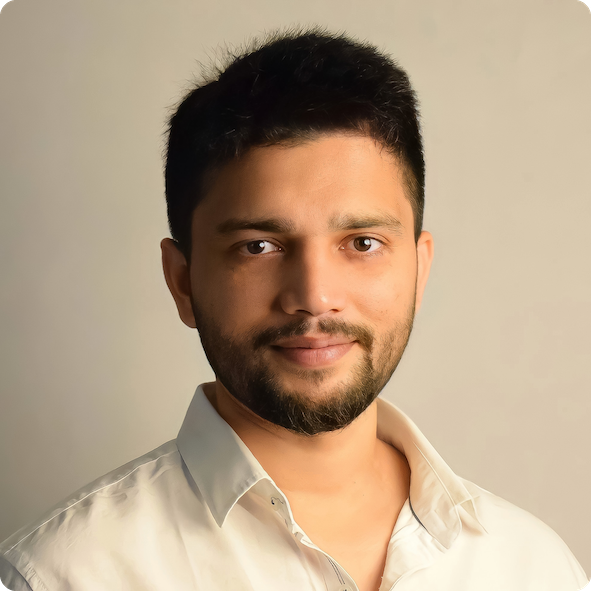
\includegraphics[width=\textwidth]{abhinav.png}
 \end{minipage}
} 

\vspace{1em} % Extra white space between the personal information section and goal

\noindent\spacedlowsmallcaps{Goal}\vspace{1em} % Goal heading, could be used for a quotation or short profile instead

\Description{Harness the power of high-performance computing to do industry-relevant research in the field of computational mechanics. Develop frameworks and algorithms to reduce computational cost and preserve solution accuracy.} % Goal text

\noindent\spacedlowsmallcaps{Research Interest}\vspace{1em} % Goal heading, could be used for a quotation or short profile instead

\Description{{Finite element analysis \ \ $\cdotp$\ \ Isogeometric analysis \ \ $\cdotp$\ \ Topology optimization \ \ $\cdotp$\ \ Phase field analysis  \ \ $\cdotp$\ \ Adaptivity \ \ $\cdotp$\ \   High performance computing}} % Goal text

%----------------------------------------------------------------------------------------
%	COMPUTER SKILLS
%----------------------------------------------------------------------------------------

\spacedlowsmallcaps{Skills Summary}\vspace{1em}

\Description{\MarginText{Languages}Python, \textsc{C++}, JavaScript, SQL, JAVA, VBA, MATLAB}

\Description{\MarginText{Tools}GIT, Docker, ParaView, Zotero, \LaTeX, Notion, Gmsh, Abaqus, COMSOL}

\Description{\MarginText{Frameworks}FEniCS, Meshio, Numpy, Pandas, Matplotlib, Plotly, pyQT, PETSc, SLEPc}

\Description{\MarginText{Platforms}Linux, Windows, macOS, Web, Android, Arduino, GCP, AWS}

\Description{\MarginText{Soft Skills}Mentoring, Collaboration, Project Management, Visual communication}

%------------------------------------------------

\vspace{1em} % Extra space between major sections
%----------------------------------------------------------------------------------------
%	EDUCATION
%----------------------------------------------------------------------------------------

\spacedlowsmallcaps{Education}\vspace{1em}

\NewEntry{2017-2023}{Indian Institute of Technology, Roorkee, India}

\Description{\MarginText{Doctor of Philosophy}\textsc{Thesis: Adaptive analysis using isoparametric and isogeometric elements}\begin{itemize}
    \item Developed framework to carry out space and time adaptivity using FEniCS.
    \item Solved fracture and topology optimization with phase field method using adaptive FEA and IGA.
    \item Developed GUI based package with support for NURBS based plate and shell isogeometric elements using python and QT.

\end{itemize}}

\NewEntry{2012-2013}{Homi Bhaba National Institute, Mumbai, India}

\Description{\MarginText{Nuclear Science and Engineering}\textsc{Orientation course on the multi-physics problems related to Nuclear power plants}}


%------------------------------------------------

\NewEntry{2010-2012}{Indian Institute of Technology, Roorkee, India}

\Description{\MarginText{Master of Technology}\textsc{Thesis: Non-Linear Analysis of RC Structure for Dynamic Loading}\begin{itemize}
    \item Validation of concrete material models in ABAQUS with experimental data.
    \item Developed python scripts for parametric simulations and post-processing.
\end{itemize}}

%------------------------------------------------

\NewEntry{2006-2010}{National Institute of Technology, Raipur, India}

\Description{\MarginText{Bachelor of Technology}\textsc{Thesis: Automated RCC design of a multistorey building using MATLAB}
\begin{itemize}
    \item Developed codes to carry out analysis and design of RCC structure.
\end{itemize}}

%------------------------------------------------

\vspace{1em} % Extra space between major sections

%----------------------------------------------------------------------------------------
%	Experience
%----------------------------------------------------------------------------------------

\spacedlowsmallcaps{Experience}\vspace{1em}

%------------------------------------------------

\NewEntry{2023}{Vanderbilt University, USA}

% \vspace{-2em}
\Description{\MarginText{Post Doctoral Fellow}\textsc{Large scale simulation of calving dynamics of Antarctic ice shelves}
\begin{itemize}
    \item Develop an adaptive phase-field algorithm for application to large-scale 3D floating ice shelves.
    \item Develop an efficient parallel code for adaptive phase-field fracture that can scale on thousands of computational cores. 
\end{itemize}}
%------------------------------------------------

%------------------------------------------------

\NewEntry{2019}{Google Summer of Code, FEniCS}

% \vspace{-2em}
\Description{\MarginText{Student Developer}\textsc{GMsh/XDMF/DOLFIN mesh processing pipeline}
\begin{itemize}
    \item Appended the \textsc{meshio} package with support for reading physical domains.
    \item Developed codes in \textsc{C++} for the mesh processing pipeline in DOLFIN-X. 
\end{itemize}}
%------------------------------------------------

\NewEntry{2013-2017}{Nuclear Power Corporation of India Limited}

\Description{\MarginText{Scientific Officer}\textsc{Analysis and design of infrastructure for nuclear power plants}
\begin{itemize}
    \item Developed codes for liquefaction analysis in VBA.
    \item Automated analysis and design of beams and columns using VBA.
\end{itemize}}


%------------------------------------------------

% \vspace{1em} % Extra space between major sections


%----------------------------------------------------------------------------------------
%	PUBLICATIONS
%----------------------------------------------------------------------------------------

\spacedlowsmallcaps{Selected Projects and Publications}\vspace{1em}

\NewEntryNoDate{An adaptive mesh refinement algorithm for phase-field fracture}

\Description{\MarginText{CMAME article (2022)}Proposed a novel methodology to carry out adaptive phase-field fracture simulation for brittle, cohesive, and dynamic fracture developed in FEniCS.}

\NewEntryNoDate{Adaptive isogeometric topology optimization using PHT-splines}

\Description{\MarginText{CMAME article (2022)}Proposed a novel methodology to carry out adaptive isogeometric topology optimization for complex, multi-patch 2D/3D design domains.}



%------------------------------------------------

% \hspace{0.75cm}
\NewEntryNoDate{Run time from 300 years to 300 min. in FEniCS}

\Description{\MarginText{FEniCS 2021 conference (2021)}Lessons learned in trying to solve medium to large scale systems with FEniCS using parallelization.}

%------------------------------------------------
\NewEntryNoDate{A 55-line topology optimization code in FEniCS}

\Description{\MarginText{arXiv article (2020)}The most compact 2D/3D topology optimization code with support for parallelization and complex design domains build with FEniCS.}

%------------------------------------------------

\NewEntryNoDate{Time adaptivity for phase field fracture in FEniCS}

\Description{\MarginText{TAFM article (2020)}Proposed a novel sub-stepping algorithm for time adaptivity to solve the problem of brittle fracture with the phase field method.}

%------------------------------------------------


% \NewEntryNoDate{\textsc{eigenplus.com} interactive educational apps}

% \Description{\MarginText{Interactive apps (2017)}Interactive android apps with accompanying blog posts to teach the concepts of structural engineering.}

%------------------------------------------------

% \vspace{1em} % Extra space between major sections



%----------------------------------------------------------------------------------------
%	OTHER INFORMATION
%----------------------------------------------------------------------------------------

\spacedlowsmallcaps{Other Information}\vspace{1em}

\Description{\MarginText{Achievements and Awards}2022 \ \ $\cdotp$\ \ \textsc{eigenplus.com} interactive educational apps reached 500K downloads}

\vspace{-0.5em} % Negative vertical space to counteract the vertical space between every \Description command

\Description{2020 \ \ $\cdotp$\ \ Developed the 55-line topology optimization code with FEniCS}

\vspace{-0.5em} % Negative vertical space to counteract the vertical space between every \Description command

\Description{2019 \ \ $\cdotp$\ \ Successfully completed Google summer of code 2019 with FEniCS}

\vspace{-0.5em} % Negative vertical space to counteract the vertical space between every \Description command

\Description{2018 \ \ $\cdotp$\ \ Got third place in "Google - Techstars Startup Weekend"}

\vspace{-0.5em} % Negative vertical space to counteract the vertical space between every \Description command

\Description{2018 \ \ $\cdotp$\ \ Developed interactive cross-platform 3D app for isogeometric analysis}

\vspace{-0.5em} % Negative vertical space to counteract the vertical space between every \Description command

\Description{2017 \ \ $\cdotp$\ \ HP Higher education award, Himachal Government, India}

\vspace{-0.5em} % Negative vertical space to counteract the vertical space between every \Description command

\Description{~~~~~~~ \ \ $\cdotp$\ \ MHRD Fellowship, Ministry of Human Resource Development, India
}

\vspace{-0.5em} % Negative vertical space to counteract the vertical space between every \Description command

\Description{2010 \ \ $\cdotp$\ \ DAE Graduate Fellowship, Board of research in nuclear science, India}

\vspace{-0.5em} % Negative vertical space to counteract the vertical space between every \Description command

\Description{~~~~~~~ \ \ $\cdotp$\ \ MHRD Fellowship, Ministry of Human Resource Development, India}

\vspace{-0.5em} % Negative vertical space to counteract the vertical space between every \Description command

\Description{2006 \ \ $\cdotp$\ \ HP board student award, Himachal Government, India}

\vspace{-0.5em} % Negative vertical space to counteract the vertical space between every \Description command

\Description{2005 \ \ $\cdotp$\ \ Developed “Fee Management System” using DBMS language FOXPRO}

\vspace{-0.5em} % Negative vertical space to counteract the vertical space between every \Description command

\Description{~~~~~~~ \ \ $\cdotp$\ \ HP board student award, Himachal Government, India}

\vspace{-0.5em} % Negative vertical space to counteract the vertical space between every \Description command

\Description{2004 \ \ $\cdotp$\ \ Certificate of Distinction, National Computer Olympiad, India}




% \Description{2013 \ \ $\cdotp$\ \ Advanced Scholarship by Gazprombank for excellent academic \newline ~~~~~~~achievements}

% \vspace{-0.5em} % Negative vertical space to counteract the vertical space between every \Description command
%------------------------------------------------
%----------------------------------------------------------------------------------------
%	Languages
%----------------------------------------------------------------------------------------
\begin{comment}


\vspace{1em}

\newlength{\langbox} % Create a new length for the length of languages to keep them equally spaced
\settowidth{\langbox}{English} % Length equals the length of "English" - if you have a longer language in your list put it here

\Description{\MarginText{Languages}\parbox{\langbox}{\textsc{Rissian}}\ \ $\cdotp$\ \ \ Mothertongue}

\vspace{-0.5em} % Negative vertical space to counteract the vertical space between every \Description command

\Description{\parbox{\langbox}{\textsc{English}}\ \ $\cdotp$\ \ \ Intermediate (conversationally fluent)}

\vspace{-0.5em} % Negative vertical space to counteract the vertical space between every \Description command

\Description{\parbox{\langbox}{\textsc{French}}\ \ $\cdotp$\ \ \ Basic (simple words and phrases only)}

\vspace{1em} % Negative vertical space to counteract the vertical space between every \Description command
\end{comment}
%------------------------------------------------
%----------------------------------------------------------------------------------------
%	Interests
%----------------------------------------------------------------------------------------

\Description{\MarginText{Interests}Making music \ \ $\cdotp$\ \ Developing interactive applications\ \ $\cdotp$\ \ Scientific animations}

%----------------------------------------------------------------------------------------
%----------------------------------------------------------------------------------------
%	publications
%----------------------------------------------------------------------------------------

\spacedlowsmallcaps{List of publications and Conferences}\vspace{1em}

\Description{\MarginText{Publications}S. Saurabh, \textbf{\underline{A. Gupta}}, and R. Chowdhury. Impact of parametric variation to achieve extreme mechanical metamaterials through topology optimization. \emph{Computer Methods in Applied Mechanics and Engineering}, 2023.} 

\Description{P. Luke, \textbf{\underline{A. Gupta}}, B. Mamandlapalli, R. Chowdhury, and Vinh Phu Nguyen. A continuous field adaptive mesh refinement algorithm for isogeometric topology optimization using PHT-Splines. \emph{Computer Methods in Applied Mechanics and Engineering}, 2023.}  

% \vspace{-0.5em} % Negative vertical space to counteract the vertical space between every \Description command
% \Description{\textbf{\underline{A. Gupta}}, B. Mamandlapalli, R. Chowdhury, and A. Chakrabarti. Integrated approach for shape optimization and solar-energy capture maximization over curved shell roofs using isogeometric analysis. \emph{submitted to Computer Aided Design}, 2023.}

\Description{\textbf{\underline{A. Gupta}}, U. M. Krishnan, Tushar Kanti Mandal, R. Chowdhury, and Vinh Phu Nguyen. An adaptive mesh refinement algorithm for phase-field fracture models: Application to brittle, cohesive, and dynamic fracture. \emph{Computer Methods in Applied Mechanics and Engineering}, 2022.}   

\vspace{-0.5em} % Negative vertical space to counteract the vertical space between every \Description command

\Description{\textbf{\underline{A. Gupta}}, B. Mamandlapalli, P. Luke, R. Chowdhury, and A. Chakrabarti. Adaptive isogeometric topology optimization using PHT splines. \emph{Computer Methods in Applied Mechanics and Engineering}, 2022.}
\vspace{-0.5em} % Negative vertical space to counteract the vertical space between every \Description command



\Description{U. M. Krishnan, \textbf{\underline{A. Gupta}}, and R. Chowdhury. Adaptive phase-field modeling of brittle fracture using a robust combination of error-estimator and markers. \emph{Engineering Fracture Mechanics}, 2022.}



\vspace{-0.5em} % Negative vertical space to counteract the vertical space between every \Description command
\Description{G. Agrawal, \textbf{\underline{A. Gupta}}, R. Chowdhury, and A. Chakrabarti. Robust topology optimization of negative Poisson’s ratio metamaterials under material uncertainty. \emph{Finite Elements in Analysis and Design, 198:103649}, Jan. 2022. }



\vspace{-0.5em} % Negative vertical space to counteract the vertical space between every \Description command

\Description{T. K. Mandal, \textbf{\underline{A. Gupta}}, V. P. Nguyen, R. Chowdhury, and A. Vaucorbeil. A length scale insensitive phase field model for brittle fracture of hyperelastic solids. \emph{Engineering Fracture Mechanics}, July 2020.}

\vspace{-0.5em} % Negative vertical space to counteract the vertical space between every \Description command

\Description{\textbf{\underline{A. Gupta}}, R. Chowdhury, A. Chakrabarti, and T. Rabczuk. A 55-line code for large-scale parallel topology optimization in 2D and 3D. \emph{arXiv preprint arXiv:2012.08208}, 2020.}

\vspace{-0.5em} % Negative vertical space to counteract the vertical space between every \Description command

\Description{\textbf{\underline{A. Gupta}}, U. M. Krishnan, R. Chowdhury, and A. Chakrabarti. An auto-adaptive sub- stepping algorithm for phase-field modeling of brittle fracture. \emph{Theoretical and Applied Fracture Mechanics, 108}, Aug. 2020.}

\vspace{-0.5em} % Negative vertical space to counteract the vertical space between every \Description command



\Description{\MarginText{Conferences}\textbf{\underline{A. Gupta}}, R. Chowdhury, and A. Chakrabarti. Optimization using isogeometric analysis. In NAFED 2019, 2019.}

\vspace{-0.5em} % Negative vertical space to counteract the vertical space between every \Description command
\Description{\textbf{\underline{A. Gupta}}, R.Chowdhury, and A.Chakrabarti. Isogeometric shape optimization of concrete shell structures. In NCMDAO 2019, 2019.}

\vspace{-0.5em} % Negative vertical space to counteract the vertical space between every \Description command
\Description{\textbf{\underline{A. Gupta}}, R. Chowdhury, and A. Chakrabarti. Development of isogeometric elements. In NAFED 2020, 2020.}

\vspace{-0.5em} % Negative vertical space to counteract the vertical space between every \Description command
\Description{\textbf{\underline{A. Gupta}}, U. M. Krishnan, R. Chowdhury, and A. Chakrabarti. Run-time from 300 years to 300 min: Lessons learned in large-scale modeling in FEniCS, 2021.}

\vspace{-0.5em} % Negative vertical space to counteract the vertical space between every \Description command
\Description{U. M. Krishnan,  \textbf{\underline{A. Gupta}}, and R. Chowdhury. Working with complex meshes: The mesh processing pipeline. In FEniCS 2021, 2021.}

\vspace{-0.5em} % Negative vertical space to counteract the vertical space between every \Description command
\Description{B. Mamindlapelly,  \textbf{\underline{A. Gupta}}, P. L. Karuthedath, and R. Chowdhury. Unified isogeometric shell shape optimization workflow. In NAFED 2021, 2022.}

\vspace{-0.5em} % Negative vertical space to counteract the vertical space between every \Description command
\Description{P. L. Karuthedath,  \textbf{\underline{A. Gupta}}, B. Mamindlapelly, and R. Chowdhury. Achieving isogeometric higher-order continuity through Bezier Extraction. In NAFED 2021, 2022.}

%----------------------------------------------------------------------------------------
%	OTHER INFORMATION
%----------------------------------------------------------------------------------------
\spacedlowsmallcaps{Teaching Experience}\vspace{1em}

\Description{\MarginText{Student co-supervisions}Reinforced concrete design of framed structures. \emph{B.Tech project}, 2018}

\vspace{-0.5em} % Negative vertical space to counteract the vertical space between every \Description command

\Description{Free vibration isogeometric analysis of framed structures. \emph{M.Tech thesis}, 2019}

\vspace{-0.5em} % Negative vertical space to counteract the vertical space between every \Description command

\Description{Comparative study of molecular dynamics and phase field modeling for brittle fracture. \emph{M.Tech thesis}, 2019}

\vspace{-0.5em} % Negative vertical space to counteract the vertical space between every \Description command
\Description{Auxetic metamaterials design using topology optimization considering uncertainty in material properties. \emph{M.Tech thesis}, 2021}

\vspace{-0.5em} % Negative vertical space to counteract the vertical space between every \Description command
\Description{Comparison of Newton-Raphson method and arc length method for non-linear analysis. \emph{B.Tech project}, 2021}

\vspace{-0.5em} % Negative vertical space to counteract the vertical space between every \Description command
\Description{Nano-topology optimization of photonic metamaterial. \emph{M.Tech thesis}, 2022}

%----------------------------------------------------------------------------------------
%----------------------------------------------------------------------------------------
%----------------------------------------------------------------------------------------
\Description{\MarginText{Graduate Teaching Assistant}2018 \ \ $\cdotp$\ \ Mechanics of solids}

\vspace{-0.5em} % Negative vertical space to counteract the vertical space between every \Description command
\Description{2019 \ \ $\cdotp$\ \ Finite element method \hspace{2.5mm} 2019 \ \ $\cdotp$\ \ Introduction to STAAD Pro}

\vspace{-0.5em} % Negative vertical space to counteract the vertical space between every \Description command
\Description{2019 \ \ $\cdotp$\ \ Introduction to C++ \hspace{6mm}  2019 \ \ $\cdotp$\ \ Numerical methods with Python}
\end{cv}

\end{document}
